\chapter{Hyperdimensional embeddings on the level of amino acids}
From here on, every hyperdimensional vector is made to be 10000-dimensional and binary unless noted otherwise.
\section{Encoding biological information into a vector}
Currently, in most of the research in hyperdimensional computing, there is an emphasis on creating and assigning hyperdimensional vectors fully randomly to certain concepts. This is useful for optimizing speed and efficiency and is not a problem for many cases such as natural language processing, where it is usually assumed that a letter does not have varying degrees of similarities to other letters in the alphabet. For protein language modeling, however, this assumption is not valid since some amino acids are chemically more similar to each other than to others, but also in an evolutionary sense. It is not uncommon to spot substitutions on the level of amino acids within the same proteins between different species and to barely notice changes in structure and function. To account for this, we tried to encode the biological information of amino acids into hyperdimensional vectors.

\subsection*{Methods}
The last layer of the 3 billion-parameter ESM-2 model~\cite{esm2} of every amino acid was extracted, resulting in 1024-dimensional real-valued embeddings for every amino acid. To extend these into hyperdimensionality, a simple matrix multiplication has been employed: $A_{1x1024} \times B_{1024x10000} = C_{1x10000}$ where $A$ is an 1024-dimensional ESM-2 embedding and B a matrix of 1024 random 10000-D vectors. The resulting vectors are then min-max scaled and rounded depending on the desired nature of the vectors. These were then 

To assess these, the vectors for each amino acids are reduced in dimensionality \textit{via} PCA into 2 dimensions and then plotted as seen in figures~\ref{fig:AArand} and~\ref{fig:AAesm}. At first glance, there is not much to spot. Yet, there is significantly more variance encoded into the first two principal components of the ESM embeddings compared to the random vectors, meaning that there should be a significant amount of similarity encoded into the hyperdimensional vectors. This may be shown more clearly when used and compared in real-world problems.

\begin{figure}[H]
    \centering
    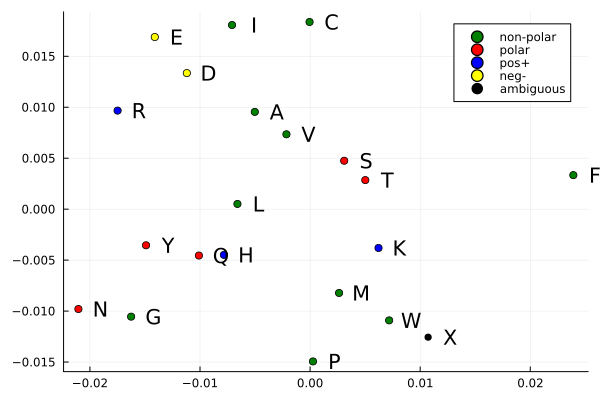
\includegraphics[scale = 0.12]{esm_emb}
    \caption{Scatter-plot of the first two principal components of ESM embeddings extended into hyperdimensionality. These PCs account for roughly 22 \% of the total variance. The amino acids are annotated and colored based on their chemical property of polarity.}\label{fig:AAesm}
\end{figure}

\section{Encoding interactions of a residue's neighborhood into a vector}
State-of-the-art protein language models have the ability to gather information on long-range dependencies around a single amino acid and encode this information into neural networks and in embeddings. To investigate the possibilities of developing embeddings on the level of amino acids, we propose a novel encoding technique within the hyperdimensional computing framework. It encodes interactions of a given amino acid in a sequence to other amino acids in its neighborhood for a predetermined range. This method thus tries to learn information about an amino acid within a sequence in an unsupervised manner. To encode the surroundings of an amino acid in a sequence, all possible pairwise interactions with the central amino acid in question in a given window were made \textit{via} binding and then all encoded into one vector \textit{via} bundling as shown figure~\ref{fig:AAtr}, starting from both random hypervectors and ESM embeddings extended into hyperdimensionality as explained earlier. This encoder was tested on the human reference proteome in UniProt, entry \textit{UP000005640}, containing 20591 proteins. After all amino acids were encoded, an element-wise average was made for every amino acid. The resulting hyperdimensional vectors were kept to a real-numbered nature to not lose information for illustration purposes.
\begin{figure}[H]
    \centering
    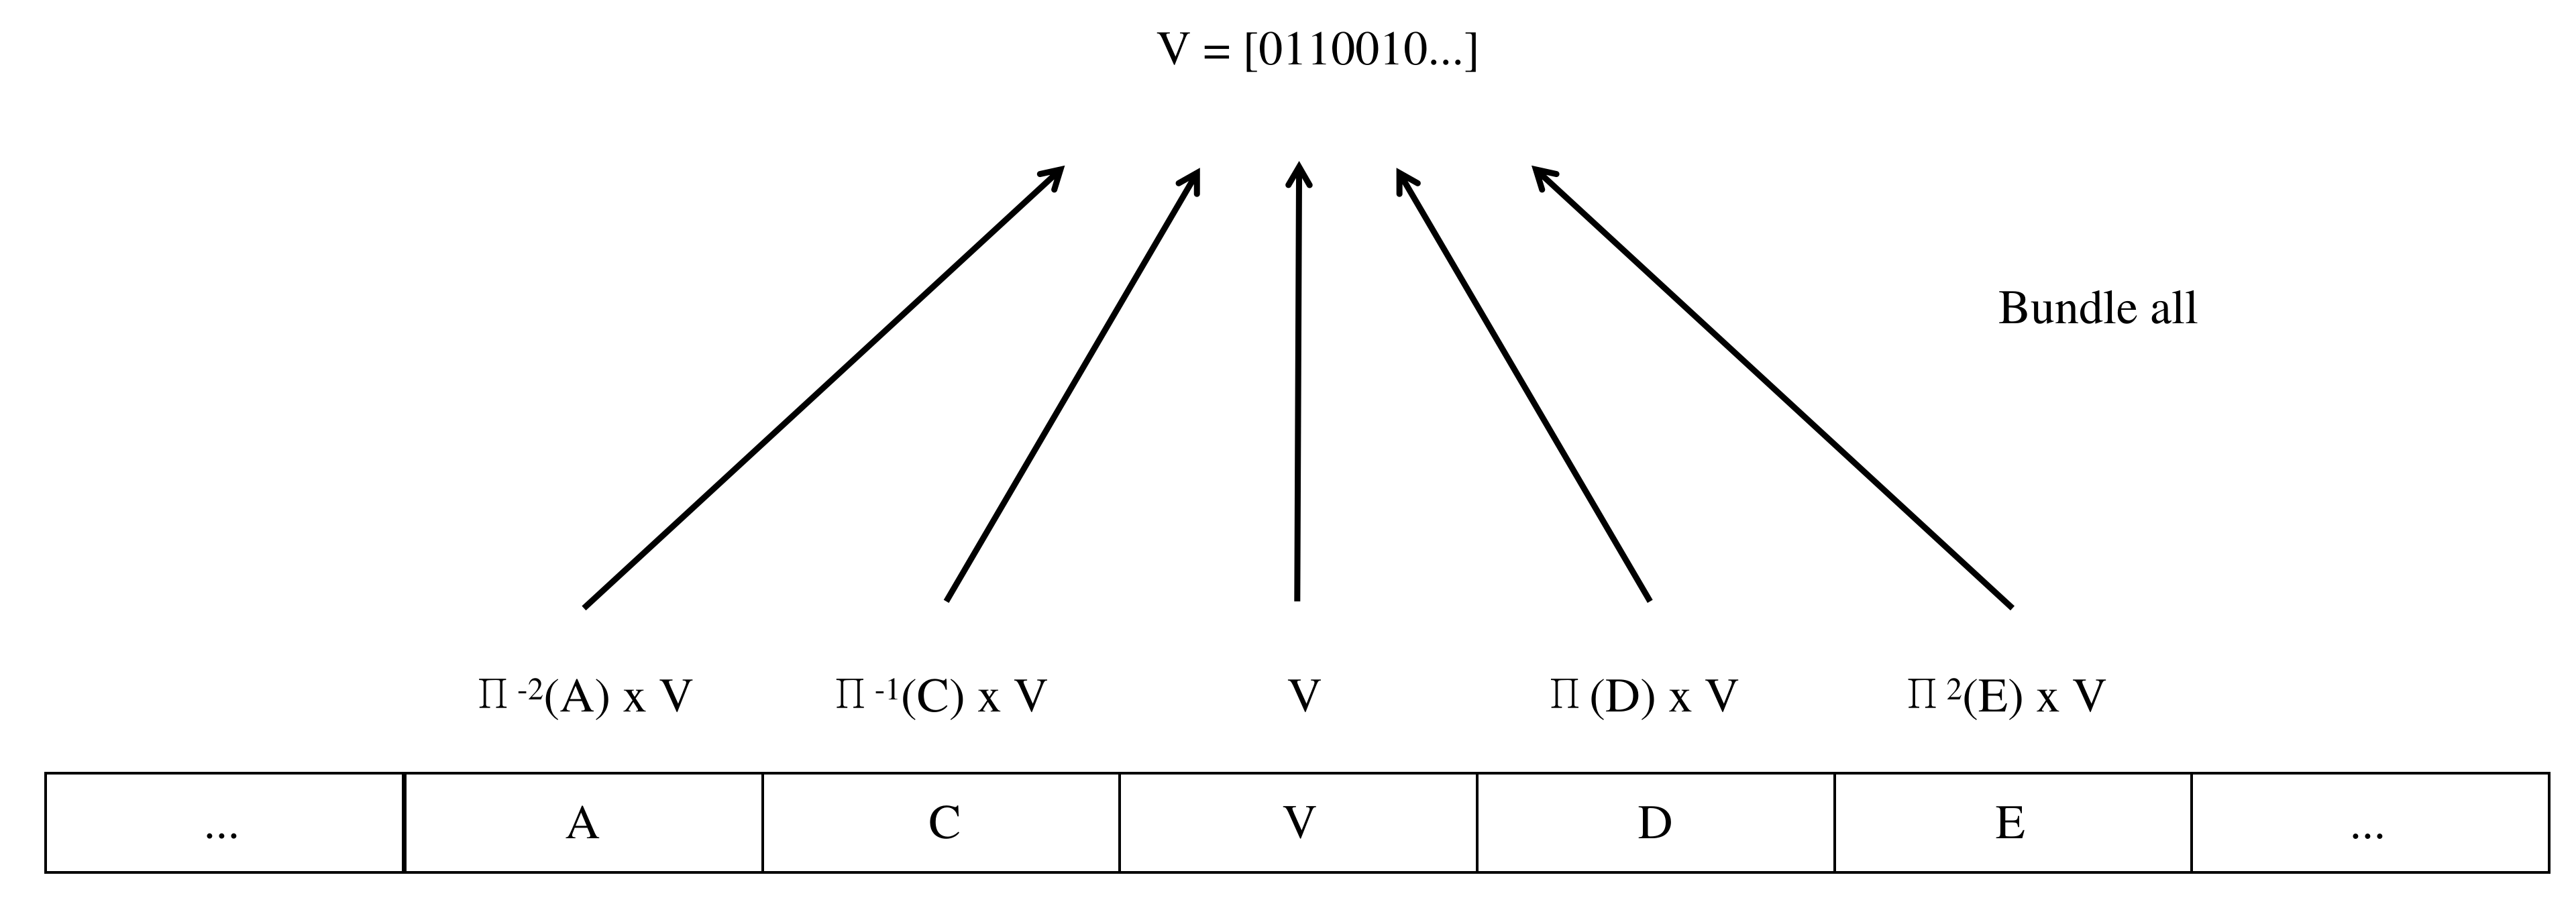
\includegraphics[scale = 0.15]{transformerlike}
    \caption{A simple demonstration of our amino acid encoder. It considers an amino acid and all amino acids in a predetermined distance (here k = 2). It produces all possible interactions of the central amino acid in the window by binding and then bundles all the pairwise interactions into one hyperdimensional vector that represents the central amino acid.}
    \label{fig:AAtr}
\end{figure}

Windows of $k = 4$ and $k = 50$ were considered for illustration purposes in figures \ref{fig:AAtr4} and \ref{fig:AAtr50}. Every single residue in the human reference proteome was encoded with information within the k-range window and an average vector was made for every amino acid. For all 20591 peptides in the reference proteome, this procedure took only 3 hours for $k = 4$, but upwards to 15 hours for $k = 50$ on a high-performance computing cluster (HPC). Both random HDVs and extended ESM embeddings were tested as base vectors. At first glance, the charged amino acids seem to be grouped vertically by PC 2, roughly dividing the polar and non-polar amino acids, albeit slightly more pronounced for $k = 50$. Also interesting, the starting ESM embeddings are extended into hyperdimensionality in a random manner, so to see very similar groupings in the PCA plots indicates that the first four amino acids before and after a residue are the most crucial.

\begin{figure}[H]
    \centering
    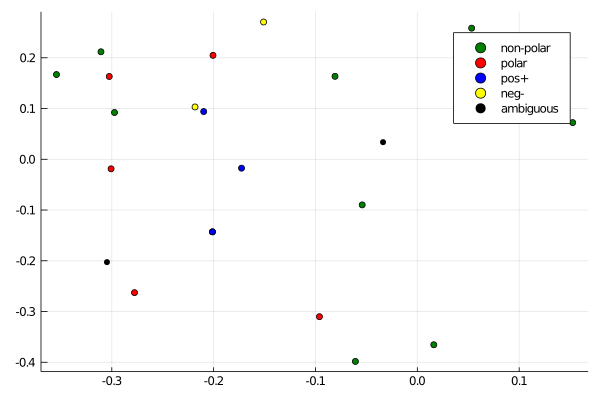
\includegraphics[scale = 0.5]{4tr_emb}
    \caption{Scatter-plot of the first two principal components of the average amino acid HDVs with neighborhood-information of $k = 4$ encoded, trained on the human reference proteome. These PCs account for roughly 21 \% of the total variance. The amino acids are annotated and colored based on their chemical property of polarity. These were made starting from extended ESM embeddings.}
    \label{fig:AAtr4}
\end{figure}

\begin{figure}[H]
    \centering
    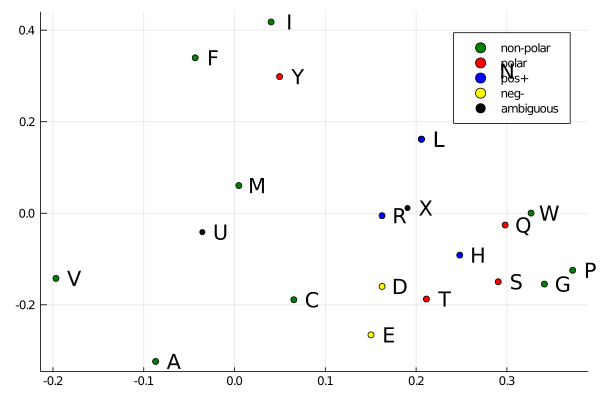
\includegraphics[scale = 0.5]{50tr_emb}
    \caption{Scatter-plot of the first two principal components of the average amino acid HDVs with neighborhood-information of $k = 50$ encoded, trained on the human reference proteome. These PCs account for roughly 21 \% of the total variance. The amino acids are annotated and colored based on their chemical property of polarity. These were made starting from extended ESM embeddings.}
    \label{fig:AAtr50}
\end{figure}

Neighborhood-encoded residue vectors were also generated as above starting from fully random HDVs for every amino acid. PCA scatter plots generated slightly different results as compared to the ones starting from ESM embeddings. These PCAs also capture less variance. For $k = 4$, some typicalities are noticed such as the close grouping of the negatively charged amino acids and the triangular grouping of H, L and R. Nonetheless, for $k = 50$ we see results deviating from all the PCA scatter plots of other neighborhood-encoded amino acids. 

\begin{figure}[H]
    \centering
    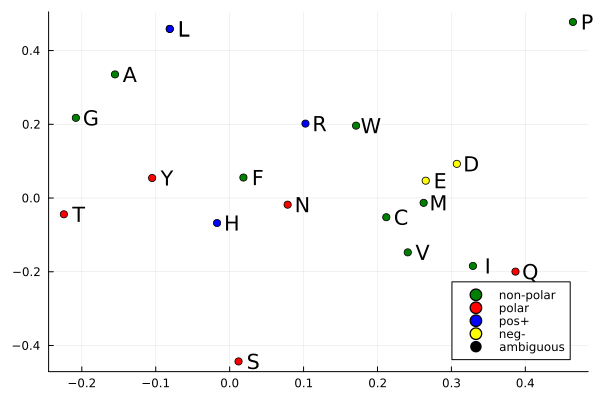
\includegraphics[scale = 0.5]{r4tr_emb}
    \caption{Scatter-plot of the first two principal components of the average amino acid HDVs with neighborhood-information of $k = 4$ encoded, trained on the human reference proteome. These PCs account for roughly 11 \% of the total variance. The amino acids are annotated and colored based on their chemical property of polarity. These were made starting from random hyperdimensional vectors.}
    \label{fig:AArtr4}
\end{figure}

\begin{figure}[H]
    \centering
    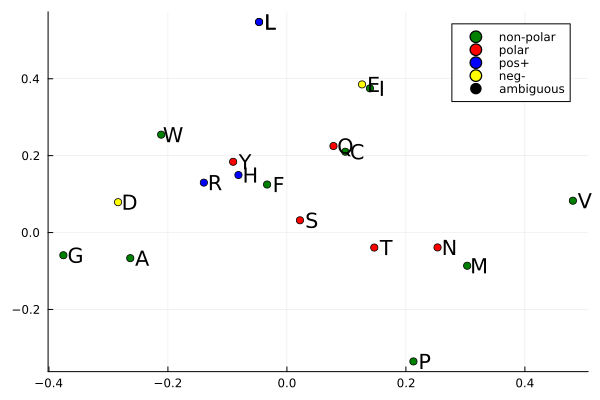
\includegraphics[scale = 0.5]{r50tr_emb}
    \caption{Scatter-plot of the first two principal components of the average amino acid HDVs with neighborhood-information of $k = 50$ encoded, trained on the human reference proteome. These PCs account for roughly 11 \% of the total variance. The amino acids are annotated and colored based on their chemical property of polarity. These were made starting from random hyperdimensional vectors.}
    \label{fig:AArtr50}
\end{figure}

In section \textit{'Learning Encodes Biochemical Properties'} of the article of Meta AI's ESM-1~\cite{esm1}, they conducted a similar experiment with their transformer model. Our results are comparable to theirs, but not as cleanly grouped which is likely due to several factors. First, the amount of data we used is not comparable to theirs: ours were trained on less than 21000 sequences whilst theirs was trained on 250 million sequences. They also included sequences originating from all recorded organisms in the UniProt database at that time whilst we confined ourselves to human sequences. Secondly, hyperdimensional vectors have a limited capacity, which is more thoroughly discussed in section~\ref{ssec:purehdc}, meaning long-range dependencies of a residue will saturate the hyperdimensional vector depending on the range. Due to the intrinsic randomness of hyperdimensional computing, it is also prone to capture some amount of noise. UMAP projections were also made, shown in section~\ref{app:chp3} in the appendices, but these did not reveal any new information. Applying these HDVs to other real-world problems should reveal the performance and usefulness of the neighborhood-encoding.